\documentclass[12pt,a4paper]{article}
\usepackage[utf8]{inputenc}
\usepackage{graphicx}
\usepackage{amsmath, amsthm, amssymb}
\usepackage[a4paper,includeheadfoot,margin=2.54cm]{geometry}
\newtheorem{theorem}{Theorem}

\begin{document}

\section{A Famous Fractal: The Koch Snowflake}

The \emph{Koch snowflake},
Helge von Koch~\cite{koch}.  
\begin{figure}[h] \label{koch}
  \centering
  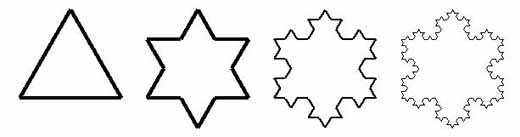
\includegraphics[width=10cm]{snowflake.jpg}
  \caption{The Koch snowflake }
\end{figure}
infinite number of times:
\begin{quote}
 \textit{First, divide.}
\end{quote}
Figure~\ref{koch}.

\begin{theorem}
  infinite length. 
\end{theorem}
\begin{proof}
  $\Delta$
  $N_i$ 
  $L_i$
  Then, 
  \begin{displaymath}
    =
    \begin{cases}
      3, & \text{if $n=0$ } \\
    \end{cases}
  \end{displaymath}
  This 
  \begin{equation}
    \label{eq:1}
    \cdot
  \end{equation}
   while  
  \begin{equation}
    \label{eq:5}
    L_n = \frac{L_{n-1}}{3} =.
  \end{equation}
  From Eqs.~\ref{eq:1}  
  \begin{displaymath}
    N_nL_n =
    \left(      \right)
    .
  \end{displaymath}
  it follows $\to \infty$, which.
\end{proof}

  The Koch snowflake has finite area. 

  
  In an iteration,, the number of new triangles $T_n$,
    Eq.~\ref{eq:1}, can be simplified to 

    \label{eq:2}

    
  $a_n$
  \begin{displaymath}
    a_0=
  \end{displaymath}
  $\Delta$, the initial equilateral triangle,, or 
  \begin{equation}
    \label{eq:3}
    a_n = \frac{a_{n-1}}{9} = \ldots .
  \end{equation}
  Eqs.~\ref{eq:2} and \ref{eq:3}
  \begin{equation*}
    b_n = = \left( \cdot 4^n \right) \left( a_0 \right)  =. 
  \end{equation*}
  total area
  \begin{align*}
    A &= a + \sum_{k=1}^n b \\
      &= a_0\left(1 + \left( \right)^k \right) \\
      &= .
   \end{align*}
  Now, since
  \begin{displaymath}
    \lim_{n} 3\left( \right) = 0,
  \end{displaymath}
  $\lim_{\to \infty} A_n$..  



\begin{thebibliography}{99}
  \bibitem{koch} Helge. \emph{Sur une courbe continue sans
      tangente, obtenue par une construction géométrique
      élémentaire.}, Arkiv,
    Kungliga Vetenskapsakademien. \textbf{1}, 681-702,.
\end{thebibliography}
\end{document}